%!TEX program = xelatex
\documentclass[dvipsnames, svgnames,a4paper,11pt]{article}
% ----------------------------------------------------
%   中山大学物理与天文学院本科实验报告模板
%   作者:Huanyu Shi,2019级
%   知乎:https://www.zhihu.com/people/za-ran-zhu-fu-liu-xing
%   Github:https://github.com/huanyushi/SYSU-SPA-Labreport-Template
%   Last update : 2023.4.10
% ----------------------------------------------------

% ----------------------------------------------------- 
%	加边框的命令
%	参考:https://tex.stackexchange.com/questions/531559/how-to-add-the-page-border-for-first-two-pages-in-latex
\usepackage{tikz}
\usetikzlibrary{calc}
\usepackage{eso-pic}
\AddToShipoutPictureBG{%
\begin{tikzpicture}[overlay,remember picture]
\draw[line width=0.6pt] % 边框粗细
    ($ (current page.north west) + (0.6cm,-0.6cm) $)
    rectangle
    ($ (current page.south east) + (-0.6cm,0.6cm) $); % 边框位置
\end{tikzpicture}}


\usepackage{xcolor}
\definecolor{c1}{HTML}{2752C9} % 目录颜色
\definecolor{c2}{RGB}{190,20,83} % 引用颜色

\usepackage{ctex}
\usepackage[top=28mm,bottom=28mm,left=15mm,right=15mm]{geometry}
\usepackage{hyperref} 
\hypersetup{
	colorlinks,
	linktoc = section, % 超链接位置,选项有section, page, all
	linkcolor = c1, % linkcolor 目录颜色
	citecolor = c1  % citecolor 引用颜色
}
\usepackage{amsmath,enumerate,multirow,float}
\usepackage{tabularx}
\usepackage{tabu}
\usepackage{subfig}
\usepackage{fancyhdr}
\usepackage{graphicx}
\usepackage{wrapfig}  
\usepackage{physics}
\usepackage{appendix}
\usepackage{amsfonts}

%
\usepackage{tcolorbox}
\tcbuselibrary{skins,breakable}
\newtcolorbox{tbox}[2][]{
    colframe=black!70!,
    breakable,
    enhanced,
	boxrule =0.5pt,
    title = {#2},
    fonttitle = \large\kaishu\bfseries,
	drop fuzzy shadow,
    #1
}
\newtcolorbox[auto counter,number within=section]{question}[1][]{
  top=2pt,bottom=2pt,arc=1mm,
  boxrule=0.5pt,
%   frame hidden,
  breakable,
  enhanced, %跨页后不会显示下边框
  coltitle=c1!80!gray,
  colframe=c1,
  colback=c1!3!white,
  drop fuzzy shadow,
  title={思考题~\thetcbcounter:\quad},
  fonttitle=\bfseries,
  attach title to upper,
  #1
}

% ---------------------------------------------------------------------
%	利用cleveref改变引用格式,\cref是引用命令
\usepackage{cleveref}
\crefformat{figure}{#2{\textcolor{c2}{图 #1}}#3} % 图片的引用格式
\crefformat{equation}{#2{(\textcolor{c2}{#1})}#3} % 公式的引用格式
\crefformat{table}{#2{\textcolor{c2}{表 #1}}#3} % 表格的引用格式


% ---------------------------------------------------------------------
%	页眉页脚设置
\fancypagestyle{plain}{\pagestyle{fancy}}
\pagestyle{fancy}
\lhead{\kaishu 中山大学物理与天文学院基础物理实验\uppercase\expandafter{\romannumeral2}} % 左边页眉,学院 + 课程
\rhead{\kaishu  \quad 光学相差实验Ⅰ} % 右边页眉,实验报告标题
\cfoot{\thepage} % 页脚,中间添加页码


% ---------------------------------------------------------------------
%	对目录、章节标题的设置
\renewcommand{\contentsname}{\centerline{\huge 目录}}
\usepackage{titlesec}
\usepackage{titletoc}
% \titleformat{章节}[形状]{格式}{标题序号}{序号与标题间距}{标题前命令}[标题后命令]
\titleformat{\section}{\centering\LARGE\songti}{}{1em}{}

% ---------------------------------------------------------------------
%   listing代码环境设置
\usepackage{listings}
\lstloadlanguages{python}
\lstdefinestyle{pythonstyle}{
backgroundcolor=\color{gray!5},
language=python,
frameround=tftt,
frame=shadowbox, 
keepspaces=true,
breaklines,
columns=spaceflexible,                   
basicstyle=\ttfamily\small, % 基本文本设置,字体为teletype,大小为scriptsize
keywordstyle=[1]\color{c1}\bfseries, 
keywordstyle=[2]\color{Red!70!black},   
stringstyle=\color{Purple},       
showstringspaces=false,
commentstyle=\ttfamily\scriptsize\color{green!40!black},%注释文本设置,字体为sf,大小为smaller
tabsize=2,
morekeywords={as},
morekeywords=[2]{np, plt, sp},
numbers=left, % 代码行数
numberstyle=\it\tiny\color{gray}, % 代码行数的数字字体设置
stepnumber=1,
rulesepcolor=\color{gray!30!white}
}




% ---------------------------------------------------------------------
%	其他设置
\def\degree{${}^{\circ}$} % 角度
\graphicspath{{./images/}} % 插入图片的相对路径
\allowdisplaybreaks[4]  %允许公式跨页 % 导入模板的相关设置
\usepackage{lipsum}
\usepackage{enumitem}
\setlist[enumerate]{label=\textup{(\arabic*)}}



%---------------------------------------------------------------------
%	正文
%---------------------------------------------------------------------

\begin{document}


\begin{table}
	\renewcommand\arraystretch{1.7}
	\begin{tabularx}{\textwidth}{
		|X|X|X|X
		|X|X|X|X|}
	\hline
	\multicolumn{2}{|c|}{预习报告}&\multicolumn{2}{|c|}{实验记录}&\multicolumn{2}{|c|}{分析讨论}&\multicolumn{2}{|c|}{总成绩}\\
	\hline
	& & & & & & & \\
	\hline
	\end{tabularx}
\end{table}


\begin{table}
	\renewcommand\arraystretch{1.7}
	\begin{tabularx}{\textwidth}{|X|X|X|X|}
	\hline
	专业:& 物理学 &年级:& 2022级\\
	\hline
	姓名:& 戴鹏辉  & 学号: & 2344016 \\
	\hline
	实验时间:& 2024/XX/XX & 教师签名:& \\
	\hline
	\end{tabularx}
\end{table}

\begin{center}
	\LARGE XXX \quad XXXXXXXXXX
\end{center}

\textbf{【实验报告注意事项】}
\begin{enumerate}
	\item 实验报告由三部分组成:
	\begin{enumerate}
		\item 预习报告:(提前一周)认真研读\underline{\textbf{实验讲义}},弄清实验原理;实验所需的仪器设备、用具及其使用(强烈建议到实验室预习),完成课前预习思考题;了解实验需要测量的物理量,并根据要求提前准备实验记录表格(第一循环实验已由教师提供模板,可以打印)。预习成绩低于10分(共20分)者不能做实验。
	    \item 实验记录:认真、客观记录实验条件、实验过程中的现象以及数据。实验记录请用珠笔或者钢笔书写并签名(\textcolor{red}{\textbf{用铅笔记录的被认为无效}})。\textcolor{red}{\textbf{保持原始记录,包括写错删除部分,如因误记需要修改记录,必须按规范修改。}}(不得输入电脑打印,但可扫描手记后打印扫描件);离开前请实验教师检查记录并签名。
	    \item 分析讨论:处理实验原始数据(学习仪器使用类型的实验除外),对数据的可靠性和合理性进行分析;按规范呈现数据和结果(图、表),包括数据、图表按顺序编号及其引用;分析物理现象(含回答实验思考题,写出问题思考过程,必要时按规范引用数据);最后得出结论。
	\end{enumerate}
	\textbf{实验报告就是将预习报告、实验记录、和数据处理与分析合起来,加上本页封面。}
	\item 每次完成实验后的一周内交\textbf{实验报告}(特殊情况不能超过两周)。
	\item 除实验记录外,实验报告其他部分建议双面打印。
\end{enumerate}


\clearpage
\tableofcontents
\clearpage

\setcounter{section}{0}
\section{XXX \quad XXXXXXXXXX \quad\heiti 预习报告}
	
\subsection{实验目的}
\begin{enumerate}
	\item 11111111111
	\item 222222222222
	\item 333333333333
	
\end{enumerate}

\subsection{仪器用具}
\begin{table}[htbp]
	\centering
	\renewcommand\arraystretch{1.6}
	% \setlength{\tabcolsep}{10mm}
	\begin{tabular}{p{0.05\textwidth}|p{0.20\textwidth}|p{0.05\textwidth}|p{0.5\textwidth}}
	\hline
	编号& 仪器用具名称 & 数量 &  主要参数(型号,测量范围,测量精度等) \\
	\hline
	1&分光计 	&1 	& KF-JJY\\

	2&平面镜 	&1 	& Φ36×4 \\
	
	3&平面透射光栅 & 1 &1/300mm \\
	
	4&汞灯&1 & GP20Ng\\
	
	5&钠灯&1 & GP20Na\\
	\hline
\end{tabular}
\end{table}

\subsection{原理概述}
%\begin{wrapfigure}{l}{0cm} % l表示靠文字内容的左侧,0cm表示环境横向长度
%	\centering
%	
\includegraphics[width=0.3\textwidth]{example.png}
%	\caption{环绕图片示例}
%\end{wrapfigure}

%\textcolor{red}{参考文献示例},参考\cite{test1,test2}。

光栅的基本原理是利用光的衍射和干涉现象,将入射的光分解为不同波长的光谱。光栅是由一系列平行的凸起和凹槽组成的结构,这些凸起和凹槽的间距非常小,一般在几微米到几毫米之间。当光线通过光栅时,会发生衍射现象,即光线会向不同的方向传播。同时,由于光栅上有许多相同的狭缝,每个狭缝都可以看作是一个次级波源(由惠更斯原理),它们发出的波会在空间中相互干涉,形成明暗相间的条纹。这些条纹称为谱线,它们的位置和强度取决于入射光的波长、光栅的间距和衍射角。任意一点的光强可由下式计算得到:
\[ I_\theta=I_0\left(\sin{\frac{\pi b\sin{\theta}}{\lambda}}\right)^2/{(\frac{\pi b\sin{\theta}}{\lambda})}^2 \]


利用分光计测量光栅常数和光线波长的方法如下:
\begin{enumerate}
	\item 调节分光计,使望远镜、平行光管和中心转轴垂直对齐,并使望远镜聚焦到无穷远。
	
	\item 将透射光栅垂直放置在载物盘上,并用平行光管照射。观察望远镜中的衍射图像,找到不同级次和不同颜色的谱线。
	
	\item 用游标盘读出各级谱线所对应的衍射角,注意消除偏心差和读数误差。
	
	\item 	根据公式 $k\lambda=d\sin{\phi}$,其中$k$是谱线级次,$\lambda$ 是入射光波长,$d$是光栅常数,$\phi$ 是衍射角,可以计算出$d$和$\lambda$ 的值。
	
	\item 如果已知入射光波长,则可以用一级谱线测出$d$的值;如果已知$d$的值,则可以用高级谱线测出$\lambda$ 的值。
\end{enumerate}


%\begin{figure}[htbp]
%	\centering
%	\subfloat[]{
%		
\includegraphics[width=0.3\textwidth]{example.png}
%	}
%	\subfloat[]{
%		
\includegraphics[width=0.3\textwidth]{example.png}
%	}
%	\subfloat[]{
%		
\includegraphics[width=0.3\textwidth]{example.png}
%	}
%
%	\subfloat[]{
%		
\includegraphics[width=0.3\textwidth]{example.png}
%	}
%	\subfloat[]{
%		
\includegraphics[width=0.3\textwidth]{example.png}
%	}
%	\subfloat[]{
%		
\includegraphics[width=0.3\textwidth]{example.png}
%	}
%	\caption{多行多列图片示例}
%\end{figure}

%\subsection{实验安全注意事项}
%\begin{enumerate}
%	\item 实验过程中,禁止汞灯光线直接照射光电管,也不宜长时间连续照射加有光阑和滤光片的光电管。\textcolor{red}{\textbf{仪器暂不使用时,均须将汞灯和光电管盒用遮光盖盖上。}}
%	\item \textcolor{red}{\textbf{ 实验过程中,禁止用眼睛直视汞灯的出射光。}}
%	\item 实验完成后,需将光电管盒的遮光盖盖上,以保护光电管。
%	\item 汞灯和电源在测量前需要预热20分钟。汞灯光源功率为50W,温度较高\textcolor{red}{\textbf{须防止烫伤。}}
%	\item 切换滤光片时直接旋转滤光器,切换光阑时需要略微向外拔出一点,旋转到需要的光阑
%	尺寸后光阑会自动复位。
%	\item 注意:切换微电流放大器档位后,需要调零,否则会影响实验精度。	
%\end{enumerate}

\subsection{实验前思考题}
\begin{question}
	简述低压汞灯的发光机理,给出特征谱线,并表明可见光波段谱线所对应的颜色。%\lipsum[10]
\end{question}
当灯管两端加上电压时,电流通过汞蒸气,使汞蒸气中的原子受到激发,从低能级跃迁到高能级,然后又从高能级跃迁回低能级,同步释放出紫外光线和可见光线。低压汞灯在可见光范围内的主要特征谱线是:579.1nm、577.0nm、546.1nm、435.8nm和404.7nm。其中546.1nm和435.8nm两条谱线较强。可见光波段谱线所对应的颜色如下表所示:

\begin{table}[htbp]
	\centering
	\begin{tabular}{|c|c|c|}
		\hline
		波长$\lambda$/nm & 颜色 \\
		\hline
		579.1 & 黄色 \\
		\hline
		577.0 & 黄色 \\
		\hline
		546.1 & 绿色 \\
		\hline
		435.8 & 蓝色 \\
		\hline
		404.7 & 紫色 \\
		\hline
		
		
	\end{tabular}
	\caption{不同波长对应的谱线颜色}
	\label{tab:mytable}
\end{table}

%\begin{question}
%	现有每厘米10000条线平面透射光栅一个,对于575nm光源,计算其+1、+2级衍射线的角度差。%\lipsum[11]
%	\tcblower
%	根据光栅衍射公式$k\lambda=d\sin{\phi}$,其中 $k$是谱线级次,$\lambda$是入射光波长,$d$是光栅常数,$\phi$是衍射角。已知每厘米10000条线的平面透射光栅,其光栅常数为 $d={10}^{-6}m$。对于575nm光源,代入公式得:
%	\[ \sin{\phi_1}=\frac{1\times575\times{10}^{-9}}{{10}^{-6}}=0.575 \]
%	\[ \sin{\phi_2}=\frac{2\times575\times{10}^{-9}}{{10}^{-6}}=1.150 \]
%	由于$\ \sin{\phi_2}$ 大于1,+2级衍射线不存在。则不存在+1、+2级衍射线的角度差。
%	
%	若换成每厘米5000条线的光栅,则光栅常数修正为$ d=2\times{10}^{-6}m$,则代入光栅衍射公式得
%	\[ \sin{\phi_1}=\frac{1\times575\times{10}^{-9}}{2\times{10}^{-6}}=0.2875 \]
%	\[ \sin{\phi_2}=\frac{2\times575\times{10}^{-9}}{2\times{10}^{-6}}=0.575 \]
%	
%	则$\mathrm{\Delta\phi}=\phi_2-\phi_1=35.10°-16.71°=18.40°$,即+1、+2级衍射角差为18.40°
%	%\lipsum[12]
%\end{question}

\begin{question}
	现有每厘米10000条线平面透射光栅一个,对于575nm光源,计算其+1、+2级衍射线的角度差。
\end{question}
	根据光栅衍射公式$k\lambda=d\sin{\phi}$,其中 $k$是谱线级次,$\lambda$是入射光波长,$d$是光栅常数,$\phi$是衍射角。已知每厘米10000条线的平面透射光栅,其光栅常数为 $d={10}^{-6}m$。对于575nm光源,代入公式得:
	\[ \sin{\phi_1}=\frac{1\times575\times{10}^{-9}}{{10}^{-6}}=0.575 \]
	\[ \sin{\phi_2}=\frac{2\times575\times{10}^{-9}}{{10}^{-6}}=1.150 \]
	
	由于$\ \sin{\phi_2}$ 大于1,+2级衍射线不存在。则不存在+1、+2级衍射线的角度差。
	
	若换成每厘米5000条线的光栅,则光栅常数修正为$ d=2\times{10}^{-6}m$,则代入光栅衍射公式得
	\[ \sin{\phi_1}=\frac{1\times575\times{10}^{-9}}{2\times{10}^{-6}}=0.2875 \]
	\[ \sin{\phi_2}=\frac{2\times575\times{10}^{-9}}{2\times{10}^{-6}}=0.575 \]
	
	则$\mathrm{\Delta\phi}=\phi_2-\phi_1=35.10°-16.71°=18.40°$,即+1、+2级衍射角差为18.40°


\clearpage
\begin{table}
	\renewcommand\arraystretch{1.7}
	\centering
	\begin{tabularx}{\textwidth}{|X|X|X|X|}
	\hline
	专业:& 物理学 &年级:& 2022级 \\
	\hline
	姓名:& 戴鹏辉 & 学号:& 22344016 \\
	\hline
	室温:& xx℃ & 实验地点: & A508 \\
	\hline
	学生签名:& & 评分: &\\
	\hline
	实验时间:& 2024/xx/xx & 教师签名:&\\
	\hline
	\end{tabularx}
\end{table}

\section{XXX \quad XXXXXXXXXX \quad\heiti 实验记录}
\subsection{实验内容和步骤}

	\subsubsection{实验一 测量光栅常数}
	
	该实验使用(已知谱线波长为$\lambda=589.4nm$的)低压钠灯为光源
	\begin{enumerate}
		\item 望远镜聚焦于无穷远(既能接受平行光),然后平行光管产生平行光,使平行光管和望远镜的光轴都垂直仪器的转轴,随后调整光栅平面与平行光管光轴垂直,光栅的刻痕与仪器转轴平行。
		
		\item 打开钠灯电源,照亮狭缝,记录主极亮的位置,即望远镜分化板竖直线与零级光谱(即平行光管狭缝像)重合时的位置,这个位置就是上一步中调节好了的位置。记下此时刻度盘两窗口的读数;
		
		\item 把望远镜向零级光谱的一边转动(如向右),直到看到一级光谱中的黄线,并使它与分化板垂直线重合。记下刻度盘两窗口读数,计算出衍射角;继续原方向转到望远镜,并在二级光谱中找到该谱线再做同样的测量;
		
		\item 把望远镜往零级光谱的另一边转动(刚才向右,现在则向左),做步骤(2)中相同测量;
		
		\item 把光栅法线左右两边所测同级光谱中的两个衍射角求平均后代入光栅衍射公式,求光栅常数。要求两个值之差不能超过10’,否则,应重新调节入射光与光栅面垂直。最后求一、二级谱线测得的光栅常数 d 的平均值及其实验不确定度。
		
	\begin{table}[htbp]
		\centering
		\begin{tabular}{|c|c|c|c|}
			\hline
			    & 主极亮位置 & +1级 & +2级 \\
			\hline
			左窗口 & 08°15′ & 358°05′ & 347°37′ \\
			\hline
			右窗口 & 188°16′ & 178°08′ & 167°39′ \\
			\hline
			    &        & -1级 & -2级 \\
			\hline
			左窗口 &      & 18°25′ & 29°03′ \\
			\hline
			右窗口 &      & 198°27′ & 209°03′ \\
			\hline
			
		\end{tabular}
		\caption{实验一测量数据}
		\label{tab:mytable}
	\end{table}
	
	\end{enumerate}

	\subsubsection{实验二 测定未知光波波长及角色散率$D$}

		以汞灯为光源,按上面方法测出各级光谱的衍射角,计算出它们的波长。然后计算角色散率及不确定度。(实际实验中测量了蓝、绿、黄三色的谱线)
		
	\begin{table}[htbp]
		\centering
		\begin{tabular}{|c|c|c|c|c|c|c|c|}
			\hline
			& 主极亮位置 & +1级 & +2级 & +1级 & +2级 & +1级 & +2级 \\
			\hline
			左窗口 & 08°14′ & 00°45′ & 353°06′ & 358°51′ & 349°12′ & 358°16′ & 348°03′ \\
			\hline
			右窗口 & 188°15′ & 180°45′ & 173°08′ & 178°53′ & 169°13′ & 178°16′ & 168°04′ \\
			\hline
			& & -1级 & -2级 & -1级 & -2级 & -1级 & -2级 \\
			\hline
			左窗口 & & 15°46′ & 23°27′ & 17°44′ & 27°25′ & 18°14′ & 28°37′ \\
			\hline
			右窗口 & & 195°47′ & 203°27′ & 197°43′ & 207°25′ & 198°16′ & 208°38′ \\
			\hline
			\multicolumn{2}{|c}{} &\multicolumn{2}{|c|}{蓝色} & \multicolumn{2}{c|}{绿色} & \multicolumn{2}{c|}{黄色} \\
			\hline
		\end{tabular}
		\caption{实验数据}
		\label{tab:data2}
	\end{table}
	
		
		
		\begin{figure}[H]
			\centering
			\includegraphics[width=9.41cm]{D:/大学各种资料/2023大二/2023大二上/基础物理实验I/5.光栅常数及光波波长的测量/SYSU-SPA-Labreport-Template-main/images/OriginalData5.jpg}
			\caption{原始实验数据}
		\end{figure}

%\subsection{实验数据记录}



%\subsection{原始数据记录}



\subsection{实验过程中遇到的问题记录}

\begin{enumerate}
	\item 	测量过程中,弯游标在转动过程中可能越过0刻度线,应当在计算时注意修正。
	
	\item 	在使用钠灯或汞灯观测黄色谱线时,理论上应存在两条,但由于分辨率问题,或二者在实际观测中距离较近,不易区分,则当作一条谱线,实际测量时,目镜中的垂直叉丝对准两谱线平均位置。
	
	\item 	在使用汞灯测量谱线时,理论上应存在紫色谱线(波长λ=404.7nm),但其强度较弱,实际观测中很难观测到,则略去,只测量蓝、绿、黄三色(即亮度最亮的三条)谱线。
	
	\item 	在目镜中观察时,有些谱线亮度较低,被环境光所影响导致难以观察,可以使用挡板遮挡部分环境光,使得观察更加容易。
	
	\item 	注意调节平行光管进光狭缝宽度至合适值,若其宽度过宽,则谱线宽度也会过宽,会降低谱线的分辨率和对比度;若其宽度过窄,会导致入射光强度减弱,使得谱线亮度不足,难以观察和测量。
	
\end{enumerate}
	

\clearpage
\begin{table}
	\renewcommand\arraystretch{1.7}
	\begin{tabularx}{\textwidth}{|X|X|X|X|}
	\hline
	专业:& 物理学 &年级:& 2022级\\
	\hline
	姓名: & 戴鹏辉 & 学号:& 22344016\\
	\hline
    日期:& 2024/xx/xx & 评分: &\\
	\hline
	\end{tabularx}
\end{table}

\section{XXX \quad XXXXXXXXXX \quad\heiti 分析与讨论}

\subsection{实验数据分析}

	\subsubsection{实验一 测量光栅常数}
		由表1中的数据,可计算得到各级衍射条纹的衍射角,如下表所示
		
		\begin{center}
			\begin{tabular}{|c|c|c|c|}
				\hline
				$\varphi_{+1}$ & $\varphi_{+2}$ & $\varphi_{-1}$ & $\varphi_{-2}$ \\
				\hline
				10°09′ & 20°37′ & 10°10′ & 20°47′ \\
				\hline
			\end{tabular}
		\end{center}

		
		则可由正负级衍射角计算平均值,并根据光栅衍射公式$k\lambda=d\sin{\varphi}$,计算光栅常数,其中钠灯的谱线已知,取$\lambda=589.4nm$,则计算结果如下表所示
		
		\begin{center}
			\begin{tabular}{|c|c|c|}
				\hline
				$\varphi_1$ & $\varphi_2$ &  \\
				\hline
				10°09′ & 20°42′ &  \\
				\hline
				$d_1$ & $d_2$ & $\overline{d}$ \\
				\hline
				$3.344\times{10}^{-6}m$ & $3.334\times{10}^{-6}m$ & $3.339\times{10}^{-6}m$ \\
				\hline
			\end{tabular}
		\end{center}

		下面计算不确定度:
		
		\begin{enumerate}
			\item  角度的重复测量引起的标准不确定度分量$u_1$,
					\[ u_1=\sqrt{\sum{(\left|\frac{\partial d}{\partial\varphi_i}\right|\sigma_i)}^2}=4.55\times{10}^{-8}m \]
					
			\item  仪器的示值误差引起的标准不确定度分量$u_2$,由分光计游标最小分度值1’,按照均匀分布考虑
					\[ u_2=\sqrt{\sum{(\left|\frac{\partial d}{\partial\varphi_i}\right|\sigma_i)}^2}=1.99\times{10}^{-7}m \]
			
			\item  合成不确定度
					\[ u_c=\sqrt{\sum{(u_i)}^2}=2.04\times{10}^{-7}m \]
			
			\item 展伸不确定度\\
					考虑正态分布,取置信概率为95\%,查表得包含因子$k=1.96$
					
					则最终测量结果表示为 $ d=\bar{d}\pm ku_c=(3.34\pm0.40)\times{10}^{-6}m$
					
					
		\end{enumerate}
		
		分析误差来源
			\begin{enumerate}
				\item 可能是由于光栅本身的刻线不均匀,或者刻线与仪器转轴不平行,导致不同级次之间的测量数据计算所得结果之间有较大误差;这是仪器本身的系统误差,无法消除,只能通过更换质量更好的光栅来避免。
				
				\item 平行光管进光狭缝的宽度可能过宽,使得入射谱线的宽度也变宽,则会降低谱线的分辨率和对比度,使得测量衍射角时不准确,从而影响计算结果。
			\end{enumerate}
		
		
		\subsubsection{实验二 测定未知光波波长及角色散率D}
			
			根据表2数据,重复实验一中的处理操作,计算正负级衍射角,计算平均值,并根据光栅衍射公式$k\lambda=d\sin{\varphi}$,计算不同衍射谱线对应光波波长,式中光栅常数取实验一中的计算结果 $d=3.34\times{10}^{-6}m$ ,则计算结果如下表所示
			
			\begin{center}
				\begin{tabular}{|c|c|c|c|}
					\hline
					\textbf{颜色} & \textbf{蓝色(b)} & \textbf{绿色(g)} & \textbf{黄色(y)} \\
					\hline
					$\varphi_{+1}$ & 07°29′ & 09°22′ & 09°58′ \\
					$\varphi_{+2}$ & 15°07′ & 19°02′ & 20°11′ \\
					$\varphi_{-1}$ & 07°32′ & 09°29′ & 10°00′ \\
					$\varphi_{-2}$ & 15°12′ & 19°10′ & 20°23′ \\
					\hline
					&  &  &  \\
					\hline
					$\varphi_1$ & 07°30′ & 09°25′ & 09°59′ \\
					$\varphi_2$ & 15°10′ & 19°06′ & 20°17′ \\
					\hline
					&  &  &  \\
					\hline
					$\lambda_1$ & 435.83nm & 546.30nm & 578.86nm \\
					$\lambda_2$ & 436.79nm & 546.29nm & 578.75nm \\
					$\overline{\lambda}$ & 436.31nm & 546.30nm & 578.80nm \\
					\hline
				\end{tabular}
			\end{center}

			下面计算不确定度:
				
			\begin{enumerate}
					\item 	角度的重复测量引起的标准不确定度分量$u_1$,
							\[ u_{b1}=\sqrt{\sum\left(\left|\frac{\partial\lambda}{\partial\varphi_i}\right|\sigma_i\right)^2}=0.402nm \]
							\[ u_{g1}=\sqrt{\sum\left(\left|\frac{\partial\lambda}{\partial\varphi_i}\right|\sigma_i\right)^2}=1.14nm \]
							\[ u_{y1}=\sqrt{\sum{(\left|\frac{\partial\lambda}{\partial\varphi_i}\right|\sigma_i)}^2}=1.36nm \]
					
					\item 仪器的示值误差引起的标准不确定度分量$u_2$,\\
							由分光计游标最小分度值1’,按照均匀分布考虑
							\[ u_{b2}=\sqrt{\sum{(\left|\frac{\partial\lambda}{\partial\varphi_i}\right|\sigma_i)}^2}=0.10nm \]
							\[ u_{g2}=\sqrt{\sum\left(\left|\frac{\partial\lambda}{\partial\varphi_i}\right|\sigma_i\right)^2}=0.13nm \]
							\[ u_{y2}=\sqrt{\sum{(\left|\frac{\partial\lambda}{\partial\varphi_i}\right|\sigma_i)}^2}=0.14nm \]
					
					\item 合成不确定度
							\[ u_{cb}=\sqrt{\sum{(u_i)}^2}=0.41nm  \quad u_{cg}=\sqrt{\sum\left(u_i\right)^2}=1.15nm  \quad u_{cy}=\sqrt{\sum{(u_i)}^2}=1.36nm \]
					
					\item 展伸不确定度
							考虑正态分布,取置信概率为95\%,查表得包含因子$k=1.96$ \\
							则最终测量结果表示为
							\[ \lambda_b=(436.31\pm0.41)nm  \quad \lambda_g=\left(546.30\pm1.15\right)nm \quad  \lambda_y=(578.80\pm1.36)nm \]
					
				\end{enumerate}
		
			将各谱线波长计算值与标准值比较(预习报告中所查得的数据),计算各谱线波长的相对误差(计算黄光谱线相对误差时,参考值取两条黄色谱线的平均波长),得到
			\[ \eta_b=\left|\frac{435.8-436.31}{435.8}\right|\times100\%=0.117\% \]
			\[ \eta_g=\left|\frac{546.1-546.30}{546.1}\right|\times100\%=0.037\% \]
			\[ \eta_y=\left|\frac{578.05-578.80}{578.05}\right|\times100\%=0.130\% \]
			
			下面计算角色散率,根据角色散率公式$D=\frac{d\theta}{d\lambda}=\frac{k}{d\cos{\theta}}$,由上表数据计算得
			
				\begin{center}
					\begin{tabular}{|c|c|c|c|}
						\hline
						\textbf{颜色} & \textbf{蓝色} & \textbf{绿色} & \textbf{黄色} \\
						\hline
						D1 & $2.98\times 10^{5} m^{-1}$ & $2.99\times 10^{5} m^{-1}$ & $3.00\times 10^{5} m^{-1}$ \\
						D2 & $6.11\times 10^{5} m^{-1}$ & $6.24\times 10^{5} m^{-1}$ & $6.29\times 10^{5} m^{-1}$ \\
						\hline
					\end{tabular}
				\end{center}


			
			下面计算角色散率的不确定度,重复上面的操作,最终包含不确定度结果如下表所示
			
			\begin{center}
				\begin{tabular}{|c|c|c|c|}
					\hline
					\textbf{颜色} & \textbf{蓝色} & \textbf{绿色} & \textbf{黄色} \\
					\hline
					D1 & $2.98 \pm 0.002 \times 10^{5} m^{-1}$ & $2.99 \pm 0.03 \times 10^{5} m^{-1}$ & $3.00 \pm 0.01 \times 10^{5} m^{-1}$ \\
					D2 & $6.11 \pm 0.07 \times 10^{5} m^{-1}$ & $6.24 \pm 0.004 \times 10^{5} m^{-1}$ & $6.29 \pm 0.10 \times 10^{5} m^{-1}$ \\
					\hline
				\end{tabular}
			\end{center}
			
			分析误差来源:
			
			\begin{enumerate}
				\item 			观察数据可发现,在测量2级谱线时,正负级衍射角的差偏大,个别数据甚至超过了10’(由于超过10’的数据是最后一组测量数据,故没有及时发现),说明光栅并未完全与平行光管光轴垂直,存在一个小角度偏差,引入了一定的系统误差。
				\item 			平行光管进光狭缝的宽度可能过宽,使得入射谱线的宽度也变宽,则会降低谱线的分辨率和对比度,使得测量衍射角时不准确,从而影响计算结果。
			\end{enumerate}
			
			
\subsection{实验后思考题}



\begin{question}
	检索文献,列举三种测量光波波长的方法,给出参考文献列表。%\lipsum[20]
\end{question}
	
	通过查阅资料,我找到了以下几种可以测量光波波长的方法:
	
\begin{enumerate}
	
	\item 	双棱镜干涉法,它利用双棱镜将单色光分成两束相干光,然后在屏幕上形成干涉条纹。通过测量条纹间距和双棱镜的夹角,可以计算出光波的波长。[1][2]
	\item 	傅里叶红外光谱仪法,它利用傅里叶变换将单色光的干涉信号转换为频率域的信号,然后通过测量信号的频率,可以计算出光波的波长。[3][4]
	\item 	激光多普勒干涉法,该方法利用激光束与一个高速旋转的多面棱镜发生多普勒效应,产生频率变化的干涉信号。通过测量干涉信号的频率差,即可求得激光波长。[5]
\end{enumerate}
	
参考文献列表:

%[1]	薛任翔. 光波波长测定方法研究[J]. 现代商贸工业, 2019, 10: 84-85. \\
%[2]	尹真, 邹淑娟, 陈娟, 权慧. 双棱镜干涉实验的深入研究[J]. 科技广场, 2014, 1: 29-34. \\
%[3]	李春明, 刘承师, 张俊峰. 测量激光波长的方法研究[J]. 激光与红外, 2007, 37(12): 1408-1410. \\
%[4]	任海萍, 王建字, 李佳戈, 等. 一种使用傅里叶红外光谱仪进行波长测量的新方法[J]. 中国药事, 2010, 24(8): 807-809. \\
%[5]	伍洲, 张文喜, 相里斌, 李杨, 孔新新. 基于多光束混合外差干涉的相位增强技术研究[J]. 物理学报, 2018, 67(2): 020601.

\begin{figure}[H]
	\centering
	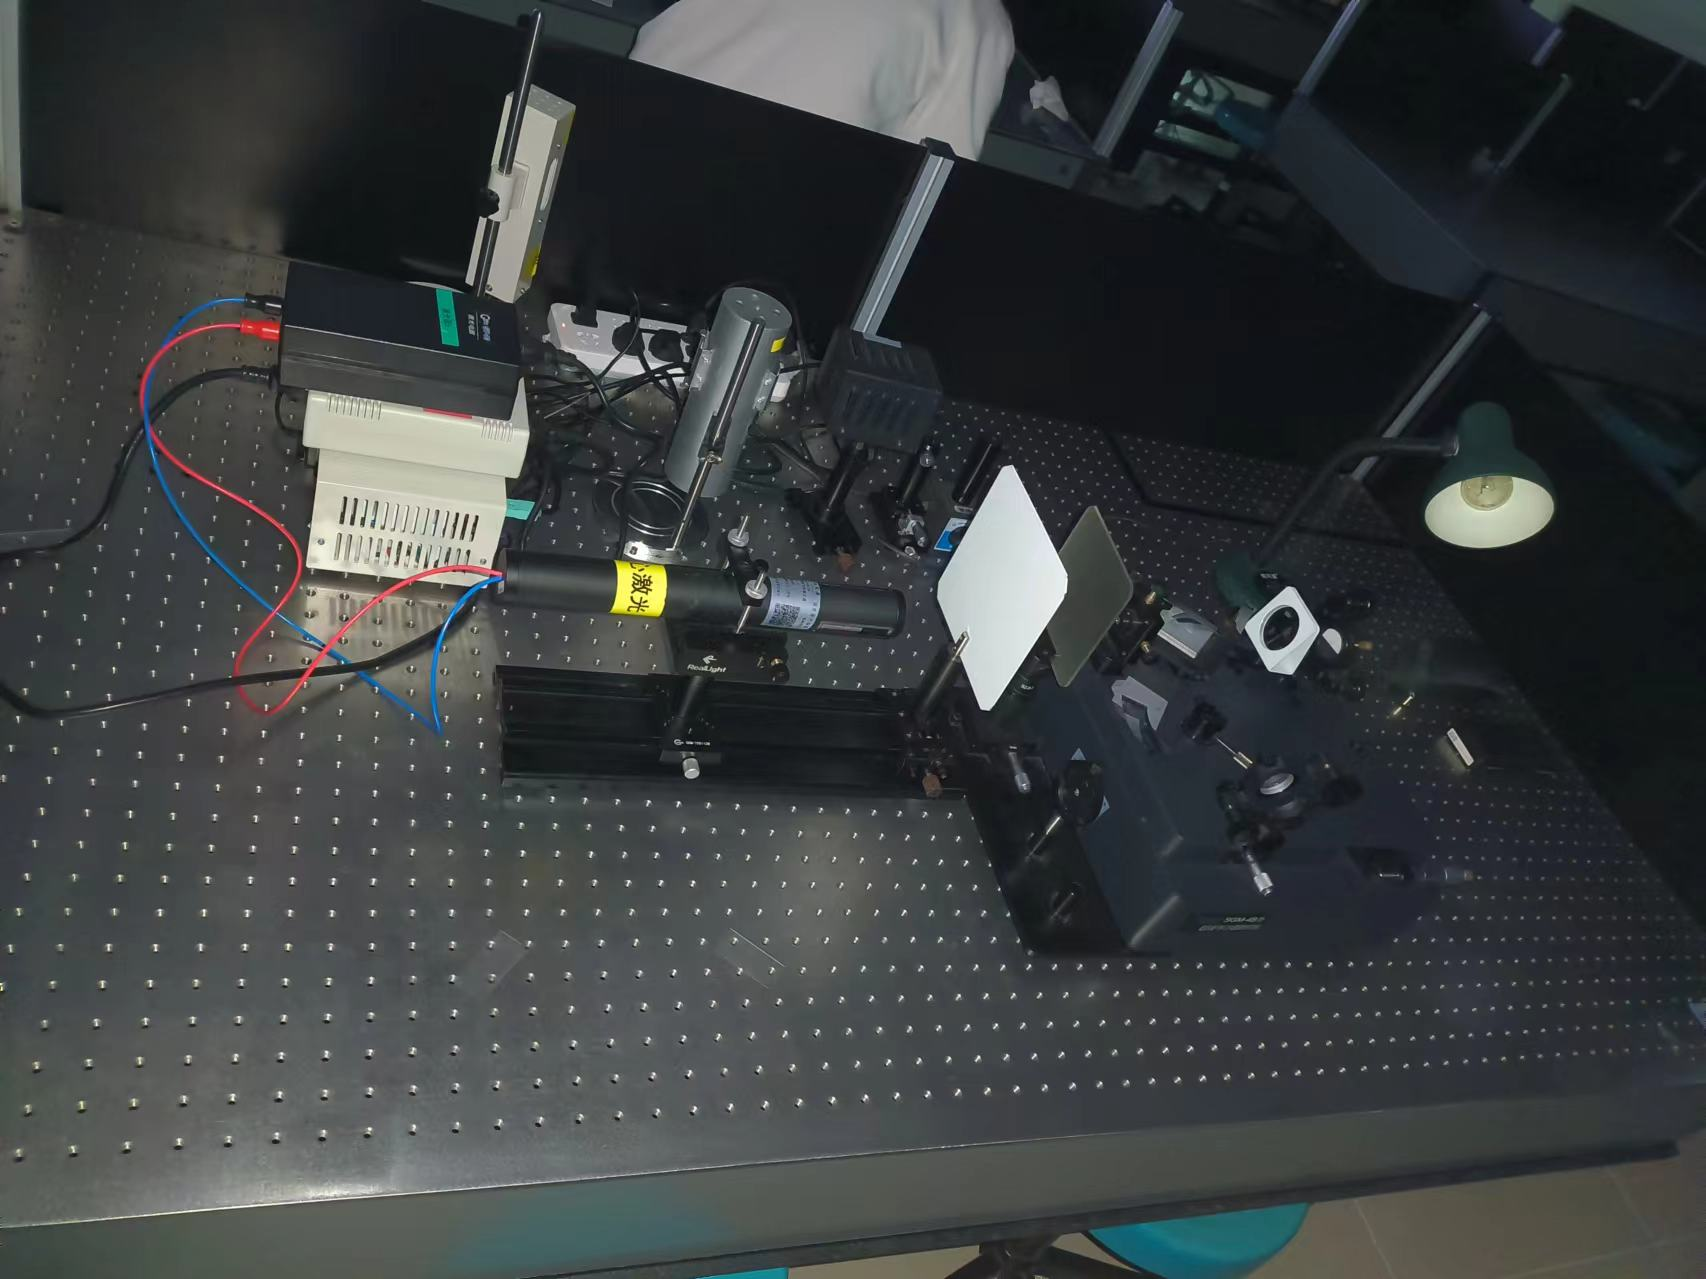
\includegraphics[width=9.41cm]{D:/大学各种资料/2023大二/2023大二上/基础物理实验I/5.光栅常数及光波波长的测量/SYSU-SPA-Labreport-Template-main/images/table.jpg}
	\caption{原始实验数据}
\end{figure}
	
\clearpage
% ---------------------------------------------------------------------
%   参考文献
%   注:使用参考文献时应按照xelatex->bibtex->xelatex->xelatex顺序进行编译
\phantomsection
\addcontentsline{toc}{section}{参考文献}
\bibliographystyle{unsrt}
\bibliography{myref}

\clearpage
\appendix
\appendixpage
\addappheadtotoc
\subsection{代码记录}
\begin{lstlisting}[style=pythonstyle,caption=代码记录示例]
	import matplotlib.pyplot as plt
	import numpy as np
	
	# Data for plotting
	t = np.arange(0.0, 2.0, 0.01)
	s = 1 + np.sin(2 * np.pi * t)
	
	fig, ax = plt.subplots()
	ax.plot(t, s)
	
	ax.set(xlabel='time (s)', ylabel='voltage (mV)',
		   title='About as simple as it gets, folks')
	ax.grid()
	
	fig.savefig("test.png")
	plt.show()
\end{lstlisting}
\begin{figure}[H]
    \centering
    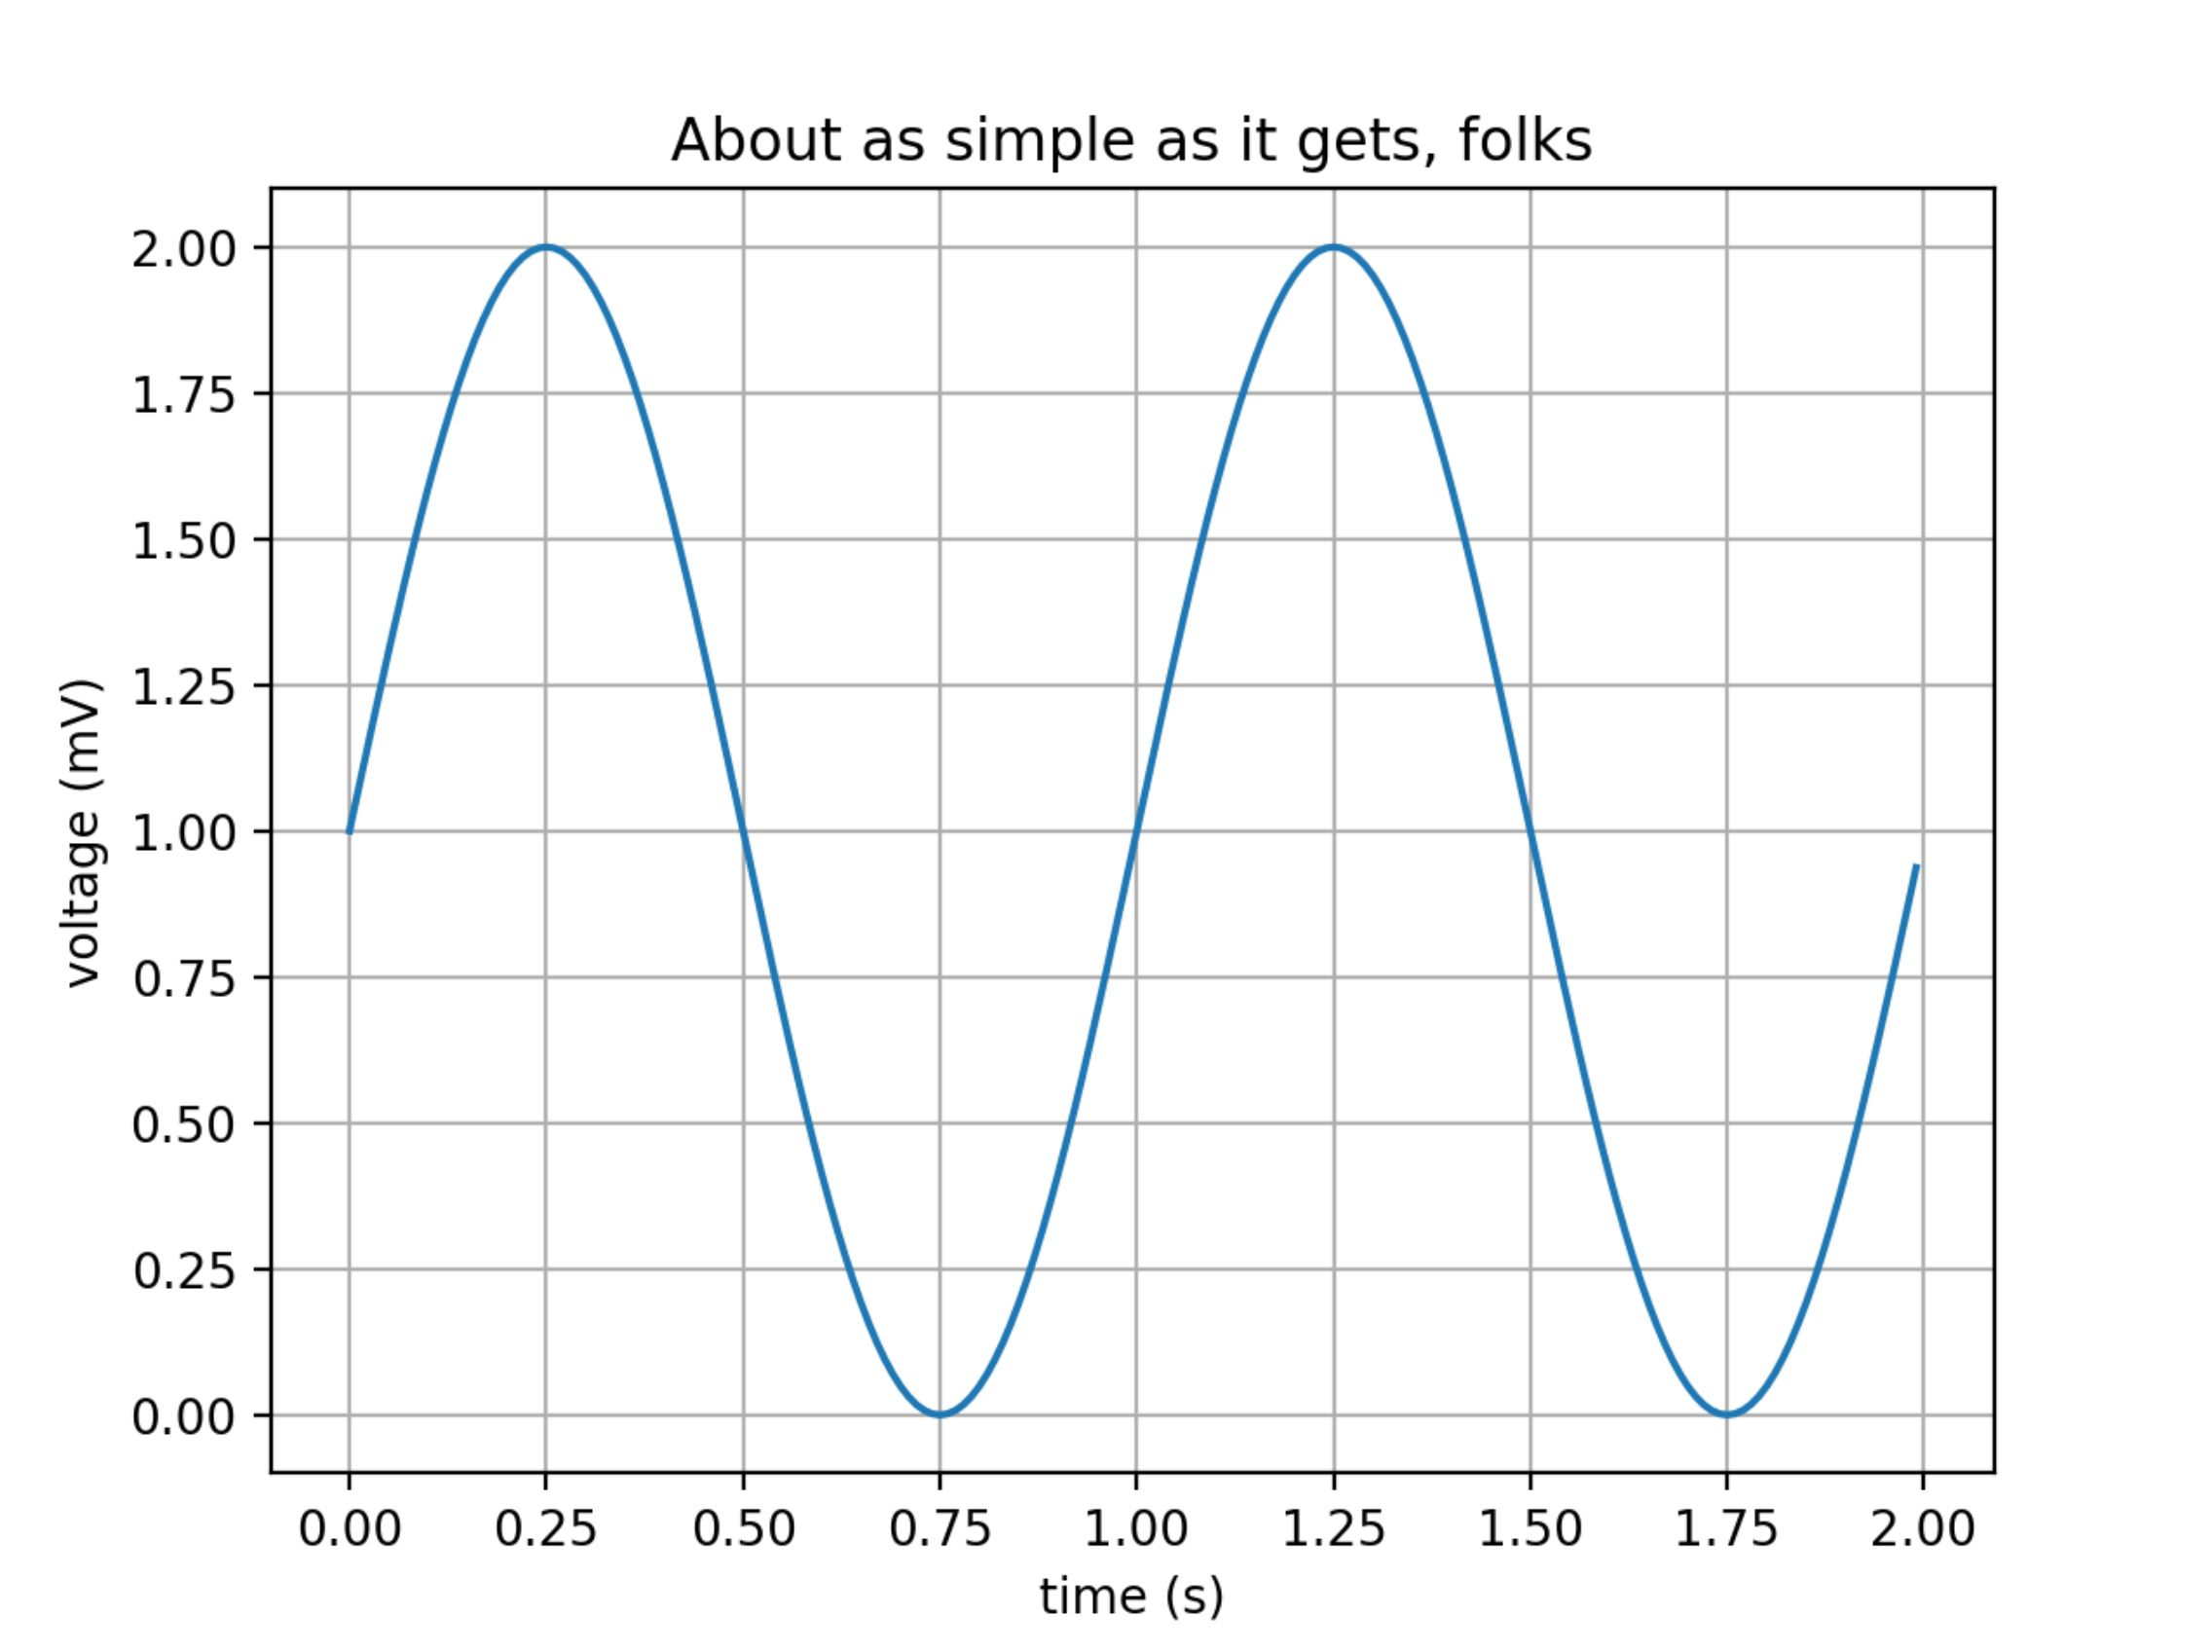
\includegraphics[width = 0.6\textwidth]{example1.png}
    \caption{Test Figure}
\end{figure}

\clearpage
\subsection{常用命令展示}
这部分将展示其他常用命令。

\begin{tbox}{颜色设置}
\begin{itemize}
	\item  \textcolor{Red}{赤}\textcolor{Orange}{橙}\textcolor{Yellow}{黄}\textcolor{Green}{绿}\textcolor{Emerald}{青}\textcolor{Blue}{蓝}\textcolor{Purple}{紫}
	\item  谁持彩练当空舞
\end{itemize}
\end{tbox}

\begin{tbox}{字号设置}
\begin{enumerate}
	\item {\LARGE 江晚正愁余}
	\item {\Large 江晚正愁余}
	\item {\large 江晚正愁余}
	\item {\normalsize 江晚正愁余}
	\item {\small 江晚正愁余}
	\item {\footnotesize 江晚正愁余}
	\item {\scriptsize 江晚正愁余}
\end{enumerate}
\end{tbox}

\begin{tbox}{字体设置(中文)}
\begin{enumerate}
	\item 宋体:{\songti 山有扶苏,隰有荷华}
	\item 仿宋:{\fangsong 山有扶苏,隰有荷华}
	\item 黑体:{\heiti 山有扶苏,隰有荷华}
	\item 楷书:{\kaishu 山有扶苏,隰有荷华}
\end{enumerate}
\end{tbox}

\begin{tbox}{Set font(English)}
\begin{enumerate}
	\item roman:\quad{\rmfamily Hello world!}
	\item sans-serif:\quad{\sffamily Hello world!}
	\item typewriter:\quad{\ttfamily Hello world!}
\end{enumerate}
\end{tbox}

\begin{tbox}{公式}
	无编号公式
    \begin{equation*}
        J(\theta) = \mathbb{E}_{\pi_\theta}[G_t] = \sum_{s\in\mathcal{S}} d^\pi (s)V^\pi(s)=\sum_{s\in\mathcal{S}} d^\pi(s)\sum_{a\in\mathcal{A}}\pi_\theta(a|s)Q^\pi(s,a)
    \end{equation*}
$$ J(\theta) = \mathbb{E}_{\pi_\theta}[G_t] = \sum_{s\in\mathcal{S}} d^\pi (s)V^\pi(s)=\sum_{s\in\mathcal{S}} d^\pi(s)\sum_{a\in\mathcal{A}}\pi_\theta(a|s)Q^\pi(s,a) $$
    有编号公式
    \begin{equation}
        J(\theta) = \mathbb{E}_{\pi_\theta}[G_t] = \sum_{s\in\mathcal{S}} d^\pi (s)V^\pi(s)=\sum_{s\in\mathcal{S}} d^\pi(s)\sum_{a\in\mathcal{A}}\pi_\theta(a|s)Q^\pi(s,a)
    \end{equation}
    \begin{equation}
        J(\theta) = \mathbb{E}_{\pi_\theta}[G_t] = \sum_{s\in\mathcal{S}} d^\pi (s)V^\pi(s)=\sum_{s\in\mathcal{S}} d^\pi(s)\sum_{a\in\mathcal{A}}\pi_\theta(a|s)Q^\pi(s,a)
    \end{equation}
	波尔文积分
    \[
    \begin{cases}
        \vspace{0.2cm}
        \displaystyle{\int_{0}^{\infty} \frac{\sin(x)}{x}\,dx = \frac{\pi}{2}}\\
        \vspace{0.2cm}
        \displaystyle{\int_{0}^{\infty} \frac{\sin(x)}{x} \frac{\sin(x/3)}{x/3}\,dx = \frac{\pi}{2}} \\
        \vspace{0.2cm}\cdot\cdot\cdot\\
        \vspace{0.2cm}
        \displaystyle{\int_{0}^{\infty} \frac{\sin(x)}{x} \frac{\sin(x/3)}{x/3} \cdot\cdot\cdot \frac{\sin(x/13)}{x/13}\,dx = \frac{\pi}{2}}\\
        \displaystyle{\int_{0}^{\infty} \frac{\sin(x)}{x} \frac{\sin(x/3)}{x/3} \cdot\cdot\cdot \frac{\sin(x/15)}{x/15}\,dx = \frac{467807924713440738696537864469}{935615849440640907310521750000}\pi}
    \end{cases}  
    \]
	多行对齐公式
\begin{align*}
    \frac{\partial}{\partial \theta_k}J(\theta) 
        &= \frac{\partial}{\partial \theta_k}\Bigg[\frac{1}{m}\sum_{k=1}^m log(1+e^{-y^{(i)}\theta^Tx^{(i)}})\Bigg] \\
        &= \frac{1}{m}\sum_{k=1}^m \frac{1}{1+e^{-y^{(i)}\theta^Tx^{(i)}}}y^{(i)}x_k^{(i)} \\
        &= -\frac{1}{m}\sum_{k=1}^m h_\theta(-y^{(i)}x^{(i)})y^{(i)}x_k^{(i)}        
\end{align*}
\end{tbox}

\begin{tbox}{引用}
	对公式的引用,如\cref{equ:test}
	\begin{equation}
        J(\theta) = \mathbb{E}_{\pi_\theta}[G_t] = \sum_{s\in\mathcal{S}} d^\pi (s)V^\pi(s)=\sum_{s\in\mathcal{S}} d^\pi(s)\sum_{a\in\mathcal{A}}\pi_\theta(a|s)Q^\pi(s,a)
		\label{equ:test}
    \end{equation}
	对图像的引用,如\cref{fig:test}
	\begin{figure}[H]
		\centering
		
\includegraphics[width=0.3\textwidth]{example.png}
		\caption{测试图片}
		\label{fig:test}
	\end{figure}
	对表格的引用,如\cref{tab:test}
	\begin{table}[H]
		\renewcommand\arraystretch{1.5}
		\caption{一个空表格}
		\begin{tabularx}{\textwidth}{|p{0.15\textwidth}|X|X|X|X|}
		\hline
		 &  &  &  &  \\    
		\hline
		 &  &  & &  \\    
		\hline
		\end{tabularx}
		\label{tab:test}
	\end{table}
\end{tbox}

\begin{tbox}{表格}
	tabular可以自己更改宽度
	\begin{table}[H]
		\renewcommand\arraystretch{1.7}
		\centering
		\caption{一个空表格}
		\begin{tabular}{|p{0.15\textwidth}|p{0.15\textwidth}|p{0.15\textwidth}|p{0.15\textwidth}|}
		\hline
		&   &  &  \\
		\hline
		 &   &  &  \\
		\hline    
		\end{tabular}
	\end{table}
	tabularx可以自适应宽度
	\begin{table}[H]
		\renewcommand\arraystretch{1.7}
		\centering
		\caption{一个空表格}
		\begin{tabularx}{\textwidth}{|p{0.2\textwidth}|X|X|X|X|X|X|}
			\hline
			& &  &  &  &  &  \\
			\hline
			 & &  &  &  &  &  \\
			\hline
		\end{tabularx}
	\end{table}
\end{tbox}
\end{document}
